\documentclass[11pt]{article}
\usepackage[margin=1in]{geometry}
\usepackage{amsmath,amssymb}
\usepackage{enumitem}
\usepackage{booktabs}
\usepackage{tikz}
\usetikzlibrary{positioning,arrows.meta}

\newcommand{\indep}{{\bot\negthickspace\negthickspace\bot}}
\DeclareMathOperator{\E}{\mathbb{E}}

\pagestyle{plain}

\begin{document}

\begin{center}
{\Large \textbf{PS200C: Quantitative Methods}} \\[6pt]
{\large In-class Activity 6: DAGs in practice}
\end{center}

\vspace{4pt}
\noindent\textbf{Name:} \hrulefill

\vspace{12pt}

\noindent Consider the DAG below.  All variables are observed.  $D$ is treatment, $Y$ is the outcome.

\begin{center}
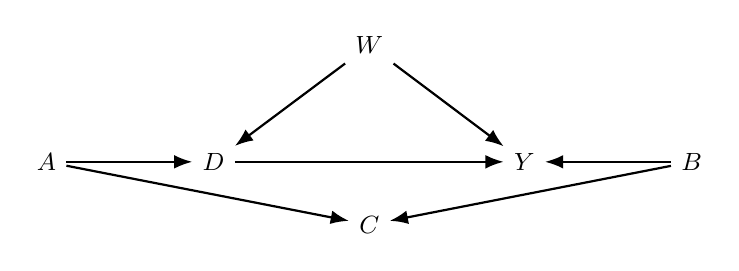
\begin{tikzpicture}[->,>=Latex,thick,node distance=1.6cm,
  every node/.style={font=\small}]
\node (W) {$W$};
\node (D) [below left = 1.0cm and 1.4cm of W] {$D$};
\node (Y) [below right = 1.0cm and 1.4cm of W] {$Y$};
\node (A) [left = 1.6cm of D] {$A$};
\node (B) [right = 1.6cm of Y] {$B$};
\node (C) [below = 1.8cm of W] {$C$};
\draw (W) -- (D);
\draw (W) -- (Y);
\draw (A) -- (D);
\draw (A) -- (C);
\draw (B) -- (Y);
\draw (B) -- (C);
\draw (D) -- (Y);
\end{tikzpicture}
\end{center}

\vspace{4pt}

%%% QUESTION 1 %%%
\noindent\textbf{Question 1: Find the backdoor paths}

\medskip
\noindent List every backdoor path from $D$ to $Y$ (any path that starts with an arrow \textit{into} $D$ and ends with an arrow into $Y$).

\vspace{3.5cm}

%%% QUESTION 2 %%%
\noindent\textbf{Question 2: Which sets satisfy the backdoor criterion?}

\medskip
\noindent For each candidate adjustment set below, say whether it would satisfy backdoor criterion (for the effect of $D$ on $Y$) and explain why or why not.  (Hint: use the backdoor paths you found in Q1.)

\begin{enumerate}[label=(\alph*), itemsep=1.8em]
\item $X = \{W\}$\\[4pt]

\item $X = \{W, C\}$ \\[4pt]

\item $X = \{W, A\}$ \\[4pt]

\item $X = \{A, C\}$ \\[4pt]
\end{enumerate}

\newpage

%%% QUESTION 3 %%%
\noindent\textbf{Question 3: Translate backdoor into CI}

\medskip
\noindent Suppose I give you an $\{X\}$ that does satisfy the backdoor criterion.  What conditional independence assumption does that imply?  Write it out in terms of $D$, $Y(d)$, and $X$.

\vspace{2.5cm}

\noindent What does the backdoor criterion have to do with understanding the various sources of association between $D$ and $Y$, and how does this relate to making a claim about the effect of $D$ on $Y$?


\vspace{5cm}

%%% BONUS %%%
\noindent\textbf{Bonus (time permitting)}: In Q2, one invalid set was invalid because conditioning on it \textit{opened} a path that was previously blocked (or, created a source of $D-Y$ association that was not previously there).   Which set, and which path?

\vspace{3cm}

\end{document}
